\chapter{Combat}
\section{Introduction to Combat}
Combat is a staple of most RPGs. 
It's intense, often exhilarating, and it gives the players a chance to strategise. Combat is essentially a series of \textit{Contests of Skill} (see section \ref{sec:contest}), but due to the nature of combat are naturally a bit more involved.
\subsection{Turns}
Combat is split into a number of turns, each turn represents about 6 seconds of in-game time, meaning 10 turns make up an in-game minute.

\paragraph{Note} One turn is the time it takes for every character to have had a go, not the time for each individual character.
\subsection{Turn Order}
To determine turn order, each player rolls $1d6+Athletics$. The turn-order is then ordered highest to lowest. Highest result goes first, lowest goes last. Any ties require a re-roll.

\paragraph{Example} Alice, Bob, and Clarice all roll for turn order. They have an athletics score of 9, 9, and 10 respectively. Alice rolls a 5, Bob rolls 3, and Clarice rolls a 6. Clarice goes first with 16, Alice is next with 14, and Bob is last with a score of 12.

\subsection{Simple Vs. Advanced Combat}
Siren supports two different styles of combat: \textit{simple}, and \textit{advanced}.

Simple combat is the most straightforward, and involves nothing more than your character sheets and your imagination. A drawn map to help visualise the space is nice, but not required.

Advanced combat, on the other hand, uses a battle mat divided into squares. This mat is used to communicate the exact position of characters and NPCs, and helps visualise movement and trajectories on the battlefield.

\subsection{Active Defence}
Active defence differs from the \textit{Defend} action in that it occurs on the attacker's turn.
There are two things a character can do when actively defending:
\begin{enumerate}
    \item \textbf{Dodge.} Roll against your \textit{Move} trait.
    \item \textbf{Parry.} Roll against half of your weapon skill, rounded down.
\end{enumerate}
You get an additional $+2$ to your roll if you also choose to move out of the way of the attack.

\newpage
\section{Simple Combat}

\subsection{Attack (Melee)}
\begin{enumerate}
    \item Roll against the appropriate weapon skill.
    \item If you succeed, the opponent gets to roll active defence.
    \item If the defence fails, roll for damage for the appropriate weapon.
\end{enumerate}

\subsection{Attack (Ranged)}
\begin{enumerate}
    \item Calculate effective skill level.
        \begin{enumerate}
            \item Target is \textbf{close}: Use base-skill.
            \item Target is at \textbf{medium} range: $Skill-3$.
            \item Target is \textbf{far}: $Skill-6$.
            \item Target is \textbf{very far}: $Skill-9$.
        \end{enumerate}
    \item Roll to attack, using the modified skill.
    \item If you succeed, target opponent may roll to dodge.
    \item If the dodge fails, roll for damage.
\end{enumerate}

\subsection{Defend}
Spend your turn doing nothing but defending. 
You get an additional $+2$ to your active defences. 
You may not attack during this turn.

\subsection{Long Action}
Any non-combat task that takes more than one turn is a \textit{long action}.
Examples of long actions could be picking a lock, untying someone, calling for backup, or applying bandages.

\subsection{Prepare Action}
Prepare an action to be triggered at a specific moment.
This can be waiting to hit someone until they're about to draw their sword, waiting for someone to turn around before hitting them in the head, or waiting for your opponent to reload their weapon before casting a spell.

\newpage
\section{Advanced Combat}
Advanced combat is much like simple combat, except it uses a battle mat. Because of this, the different possible actions in a turn are affected by this addition.

\subsection{Movement}
Particularly, the characters rely on their movement points to move about the battle mat.
Movement is 8-directional (see figure \ref{fig:directions}), and moving in any direction costs 1 movement point.

\begin{figure}
    \centering
    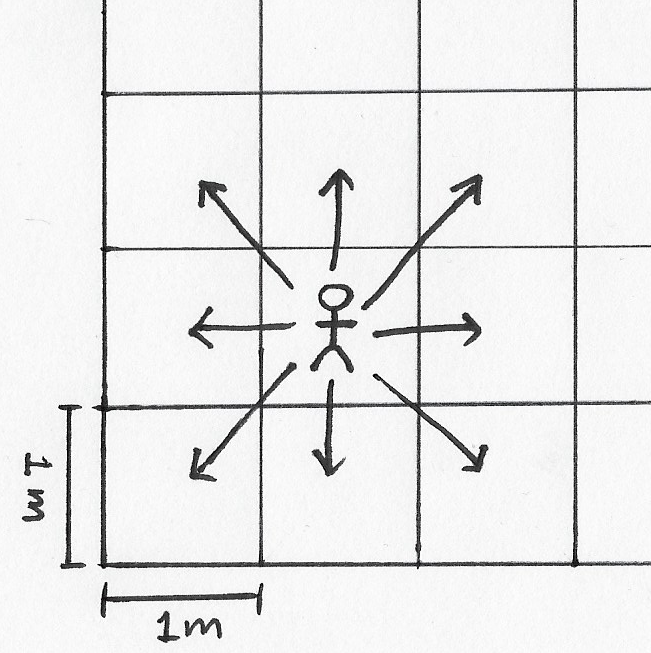
\includegraphics{graphics/directions.png}
    \caption{The eight movement directions}
    \label{fig:directions}
\end{figure}

Your character can only move as far as their movement points allow, but you may choose to move a shorter distance if you so desire. Figure \ref{fig:movement} shows an example of a character moving 4 squares, which is worth 4 movement points.

\begin{figure}
    \centering
    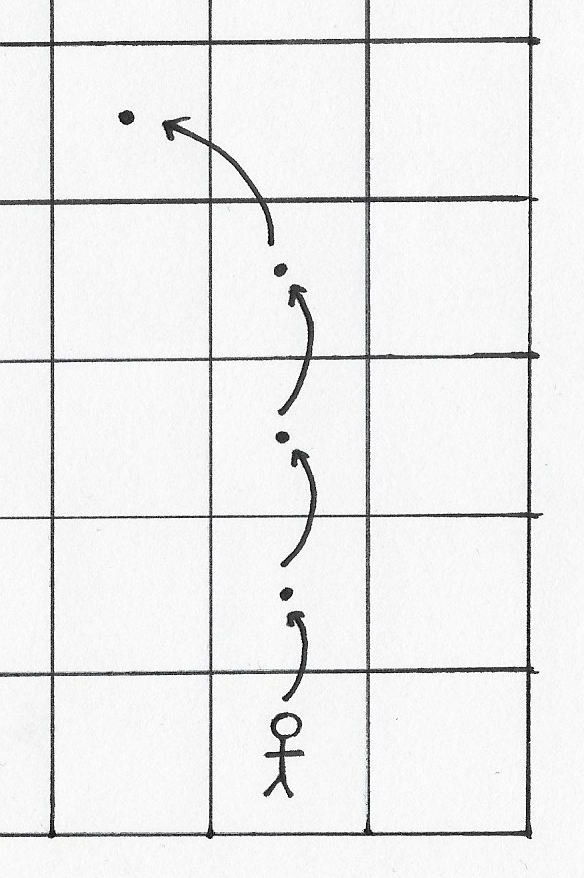
\includegraphics{graphics/movement.png}
    \caption{Example of movement.}
    \label{fig:movement}
\end{figure}

\subsection{The Grid}
The battle mat is subdivided into a grid of squares. 
The in-game size of a square is $1m^2$, although the GM may scale it up or down as necessary.
The GM must alert the players of the scale if it differs from the standard $1m^2$.

\subsection{Actions}
\subsubsection{Long Action}

\subsubsection{Move \& Attack (Melee)}
\begin{enumerate}
    \item Move up to half your movement (rounded down) before or after attacking.
    \item Roll against the appropriate weapon skill.
    \item If you succeed, the opponent gets to roll active defence.
    \item If the defence fails, roll for damage for the appropriate weapon.
\end{enumerate}

\subsubsection{Move \& Attack (Ranged)}
\begin{enumerate}
    \item Move up to half your movement (rounded down) before or after attacking.
    \item Calculate effective skill level.
        \begin{enumerate}
            \item If target is within weapon's range, do nothing else.
            \item Subtract 3 points every time you exceed the range.
        \end{enumerate}
    \item Roll to attack, using the modified skill.
    \item If you succeed, the opponent may roll to dodge.
    \item If the dodge fails, roll for damage.
\end{enumerate}

\paragraph{Example} Will the Ranger is out hunting for his party. He spots a deer in the distance. His bow has a range of 100 metres, the deer is 300 metres away. This exceeds the bow's range twice ($2\times -3$ penalty). Will must roll $Longbow-6$ to succeed.

\subsubsection{Move \& Defend}
Move up to half your movement (rounded down) before defending. 
Spend the rest of your turn doing nothing else. 
You get an additional $+2$ to your active defences. 
You may not attack during this turn.

\subsubsection{Prepare Action}
Prepare an action to be triggered at a specific moment.
This can be waiting to hit someone until they step into the square in front of you, waiting for your opponent to reload their weapon before casting a spell, or waiting for a party member to stand in the square next to you before charging at the enemies.

\subsubsection{Relocate}
Move as far as your movement score allows and do nothing else.
Roll \textit{Athletics} to run, this doubles your range if you succeed.
If you fail you trip and fall prone.
If prone you may try to get up again on your next turn.